\scanpage{55}
% archive foliation: 54
\margin{\illegible{1}}
XVIII\qquad L e s\quad é p o u s a i l l e s\qquad (2)

J'ai scruté et j'ai fouillé - par pleines brassées je ramasse tout à l'entour les paires enlacées disant un même message. Pêle-mêle je les jette devant moi ...

Puis, comme un enfant appliqué intensément enfile collier de pierres multicolores qu'il \unsure{assem\deleted{t}ble} à son gré - sans en laisser une seule, car toutes lui semblent belles ! ... lestement passant les unes, et sur d'autres s'arrêtant longement pour les contempler à loisir ... ainsi du chaos chatoyant de mes trouvailles je prépare ce collier - m o n collier - pour te l'offrir ... et \deleted{pour} l'oublier ...

Le jeu était p l a i s i r - il était découverte ! Qu'importe s'il reste \deleted{\unsure{collier}} \inserted{trace} pour témoigner du jeu \inserted{révolu} d'un enfant qui découvre \unsure{!} Quel sens a un collier, si ce n'est le plaisir de le faire ...

Ou ... susciter en \uline{toi} d é s i r de scruter et fouiller - de ramasser toi-même perles et pierres par poignées ... contempler longuement une à une celles qui t e \unsure{s} parlent, et au gré de \deleted{ta} \inserted{\uline{ton} « \unsure{désir} »} \deleted{fantaisie} assembler t o n collier ?

\deleted{A quoi bon un collier qui ne suscite désir d'en faire un plus beau ?}

Je termine d'un deuxième rang de paires enlacées ... \unsure{Si} le jeu \unsure{te} plait encore, \deleted{tu peux} regarde\deleted{r} faire ... ou \deleted{tu peux} fai\deleted{re}\inserted{s} \inserted{en un plus beau.}

11. En les choses de la Création s'enlacent et s'unissent :

\begin{flushleft}
l u m i è r e\quad et\quad o m b r e\\
le clair et l'obscur\\
le jour et la nuit\\
le brillant et le terne

savoir et mystère\\
le connu et l'inconnu\\
le connaissable et l'inconnaissable\\
connaissance et ignorance

le précis et le vague\\
le particulier et le général
\end{flushleft}

\figure{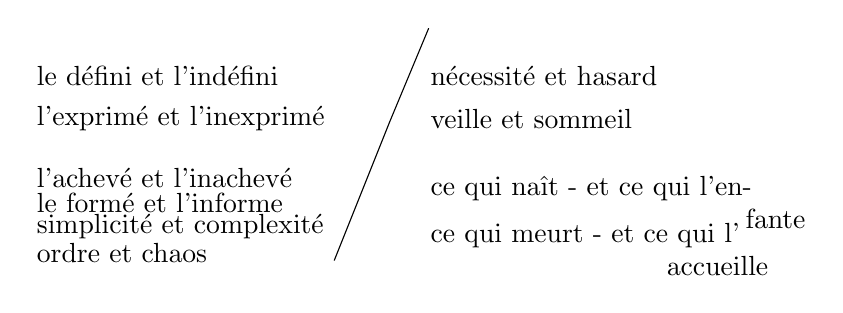
\begin{tikzpicture}[x=1cm,y=1cm]
\node[anchor=west] at (0,0) {le défini et l'indéfini};
\node[anchor=west] at (0,-.55) {l'exprimé et l'inexprimé};
\node[anchor=west] at (0,-1.3) {l'achevé et l'inachevé};
\node[anchor=west] at (0,-1.62) {le formé et l'informe};
\node[anchor=west] at (0,-1.92) {simplicité et complexité};
\node[anchor=west] at (0,-2.25) {\unsure{ordre et chaos}};
\draw (5.1,.6)--(4.6,-.6)--(3.9,-2.35);
\node[anchor=west] at (5,0) {nécessité et hasard};
\node[anchor=west] at (5,-.55) {veille et sommeil};
\node[anchor=north west,align=left] at (5,-1.15) {ce qui naît - et ce qui l'en-\\\hspace{4cm}fante};
\node[anchor=north west,align=left] at (5,-1.75) {ce qui meurt - et ce qui l'\\\hspace{3cm}\unsure{accueille}};
\end{tikzpicture}}
